\chapter{QCD at hadronic colliders}
\label{chap:theory}

\section{The QCD Lagrangian}

	The Lagrangian for QCD is more complicated than the one previously seen for QED.  This is in part due to us having to sum over different representations of the generating group, $SU(3)$, but mainly because the fields no longer commute with one another (they are non-Abelian in nature) and this leads to gauge boson self-interactions.  The full Lagrangian is as follows ~\cite{muta} \footnote{With the bare quantity subscripts supressed}:

	\begin{subequations}
	\begin{equation}
	\mathcal{L}^{QCD}=\overline{\psi}^i\left(i\slashed D^{ij}-m\delta^{ij}\right)\psi^j - \frac{1}{4}F^a_{\mu\nu}F^{a\mu\nu} - \frac{1}{2\xi}(\partial^\mu A_\mu^a)^2 + (\partial^\mu\chi^{a*})\mathcal{D}_{\mu}^{ab}\chi^b.
	\end{equation}
	\begin{equation}
	D_\mu^{ij} = \delta^{ij}\partial_\mu - ig_s(T^c)^{ij}A^c_\mu.
	\end{equation}
	\begin{equation}
	\mathcal{D}_\mu^{ab} = \delta^{ab}\partial_\mu - g_sf^{abc}A^c_\mu.
	\end{equation}
	\end{subequations}

	where the indices $i$, $j$ run from 1 to 3, the indices $a$, $b$, $c$ run from 1 to 8, $D_\mu$ is the covariant derivative in the fundamental representation, $\mathcal{D}_{\mu}$ is the covariant derivative in the adjoint representation, $T^a$ are the generating matrices and finally $f^{abc}=i(T^a_{adj})^{bc}$.  The $\chi$ fields are the `ghost' excitations and their origin will be explained in section 3.1.\\In analogy to section (2) we begin by decomposing equation (12) into a free Lagrangian and an interacting Lagrangian as follows:

	\begin{equation}
	\mathcal{L}_0^{QCD} = \overline{\psi}^i\left(i\slashed \partial-m\right)\psi^i - \frac{1}{4}\partial_{[\mu}A_{\nu]}^a\partial^{[\mu}A^{\nu]a} - \frac{1}{2\xi}(\partial^\mu A_\mu^a)(\partial^\nu A_\nu^a) + (\partial^\mu \chi^{a*})(\partial_\mu \chi^a),
	\end{equation}

	\begin{equation}
	\mathcal{L}_{I}^{QCD} = g_s\overline{\psi}^i T^a_{ij}\gamma^\mu\psi^j-\frac{g_s}{2}f^{abc}\partial_{[\mu}A^a_{\nu]}A^{b\mu}A^{c\nu}-\frac{g_s^2}{4}f^{abe}f^{cde}A^a_\mu A^b_\nu A^{c\mu}A^{d\nu}-g_sf^{abc}\partial^\mu\chi^{a*}\chi^bA^c_\mu.
	\end{equation}

	By calculating the QCD partition function and acting with the appropriate derivatives we can find the fermion propagator and the ghost propagator, repectively:

	\begin{equation}
	\langle0|\psi_i(x)\psi_j(y)|0\rangle = S_F(x-y) = \int \frac{d^4k}{(2\pi)^4}e^{-ik\cdot(x-y)}\delta_{ij}\frac{i}{\slashed k - m +i\epsilon},
	\end{equation}
	\begin{equation}
	\langle0|\chi_a(x)\chi_b(y)|0\rangle = H_F(x-y) = \int \frac{d^4k}{(2\pi)^4}e^{-ik\cdot(x-y)}\delta_{ab}\frac{i}{k^2+i\epsilon}.
	\end{equation}

	and we can read off the various QCD vertex factors directly from the interaction Lagrangian.

	\subsection{The Faddeev-Popov Procedure for NAGTs}

	All that remains to be done is to evaluate the gluon propagator.  As in QED when trying to compute the propagator of a massless gauge boson we can use the work of Faddeev and Popov.  The functional integral we want to evaluate is in the form:

	\begin{equation}
	\int DAe^{-\frac{i}{4}\int d^4xF^a_{\mu\nu}F^{a\mu\nu}}.
	\end{equation}

	Where $DA=\prod_x\prod_{a, \mu}dA^a_\mu$.  As briefly outlined above we would like to perform a functional integration over all possible gauge choices and then pick out the subset of gauges we are interested in by enforcing the gauge condition $G(A)=0$ to eliminate overcounting.  This constraint may be written as ~\cite{p&s}:

	\begin{equation}
	\int D\alpha(x)\delta(G(A^\alpha))Det\left(\frac{\delta G(A^\alpha)}{\delta\alpha(x)}\right) = 1.
	\end{equation}

	Where $A^\alpha_\mu = A_\mu - \frac{1}{g_s}\partial_\mu\alpha(x)$.  Making a gauge transformation ($A_\mu\rightarrow A^\alpha_\mu$) and inserting equation (18):

	\begin{subequations}
	\begin{equation}
	\int DAe^{-\frac{i}{4}\int d^4F^a_{\mu\nu}F^{a\mu\nu}} = \int DA\int D\alpha(x)\delta(G(A^\alpha))Det\left(\frac{\delta G(A^\alpha)}{\delta\alpha(x)}\right)e^{-\frac{i}{4}\int d^4F^a_{\mu\nu}F^{a\mu\nu}},
	\end{equation}
	\begin{equation}
	= \int D\alpha(x)\int DA\delta(G(A^\alpha))Det\left(\frac{\delta G(A^\alpha)}{\delta\alpha(x)}\right)e^{-\frac{i}{4}\int d^4F^a_{\mu\nu}F^{a\mu\nu}}.
	\end{equation}
	\end{subequations}

	We are free to change the functional integration variable to $A_\mu^\alpha$ since everything is gauge invariant leading to an integrand which \emph{only} depends on $A^\alpha_\mu$.  We can therefore simply relabel back to $A_\mu$:

	\begin{equation}
	= \left(\int D\alpha(x)\right)\int DA\delta(G(A))Det\left(\frac{\delta G(A)}{\delta\alpha(x)}\right)e^{-\frac{i}{4}\int d^4F^a_{\mu\nu}F^{a\mu\nu}}.
	\end{equation}

	The functional integration can now just be factored out as a constant and we can choose the function $G(A)$ as a generalisation of the Lorentz gauge: $G(A)=\partial^\mu A^a_\mu-\omega^a$.  This choice leads us to the correct gluon propagator - along with our free parameter, $\xi$:

	\begin{equation}
	\langle0|A_a(x)A_b(y)|0\rangle = G_F^{\mu\nu}(x-y) = \int \frac{d^4x}{(2\pi)^4}e^{-ik\cdot(x-y)}\delta_{ab}\frac{-i}{k^2+i\epsilon}\left(g^{\mu\nu}-(1-\xi)\frac{k^\mu k^\nu}{k^2}\right).
	\end{equation}

	but because the QCD gauge transformation is more involved than the QED eqivalent the determinant term still depends on $A_\mu$:

	\begin{equation}
	Det\left(\frac{\delta G(A)}{\delta\alpha(x)}\right) = Det\left(\frac{\partial_\mu D^\mu}{g_s}\right).
	\end{equation}

	We can however simply invent another type of field and choose to write out determinant as

	\begin{equation}
	Det\left(\frac{\delta G(A)}{\delta\alpha(x)}\right) = \int D\chi D\overline{\chi}e^{i\int d^4x\overline{\chi}(-\partial_\mu D_\mu)\chi}.
	\end{equation}

	These non-physical modes are called the Faddeev-Popov ghosts/antighosts and are a consequence of enforcing gauge invariance - they are represented by the final term in equation (12a).

	\subsection{Renormalising the QCD Lagrangian}

	Similarly to QED we anticipate divergent quantities in our calculations above tree level and so we introduce counterterms into our Lagrangian.  Similarly to equation (4) we have the following relations:

	\begin{subequations}
	\begin{equation}
	\psi_0 = Z_\psi^\frac{1}{2}\psi,  \hspace{15mm}  A_0^a = Z_A^\frac{1}{2}A^a,  \hspace{15mm}  \chi^a_0 = Z_\chi^\frac{1}{2}\chi^a,
	\end{equation}
	\begin{equation}
	m_0 = Z_mm,  \hspace{15mm}  g_{s0} = Z_sg_s,  \hspace{15mm}  \xi_0 = Z_\xi\xi.
	\end{equation}
	\end{subequations}

	Inserting these into equations (13) and (14) and rearranging so that we have $\mathcal{L^{QCD}} = \mathcal{L}_0 + \mathcal{L}_{ct}$ where $\mathcal{L}_0$ is as definied in equation (13) and the counterterm Lagrangian is:

	\begin{equation}
	\begin{split}
	\mathcal{L}_{ct} = &-(Z_A - 1)\frac{1}{4}(F^a_{\mu\nu})^2 + (Z_\chi - 1)i(\partial^\mu\chi^a)(\partial_\mu\chi^a) + (Z_\psi - 1)\overline{\psi^i}(i\slashed \partial - m)\psi^i - Z_\psi(Z_m - 1)m\overline{\psi^i}\psi^i + \ldots \\
	&-(Z_sZ_A^\frac{3}{2}-1)\frac{1}{2}g_sf^{abc}\partial_{[\mu]}A^a_{\nu]}A^{b\mu}A^{c\nu} - (Z_s^2Z^2_A - 1)\frac{1}{4}g_s^2f^{abe}f^{cde}A^a_\mu A^b_\nu A^{c\mu}A^{d\nu} - \ldots \\
	&-(Z_sZ_\chi Z_A^\frac{1}{2} - 1)ig_sf^{abc}(\partial^\mu\chi^a)\chi^bA^c_\mu + (Z_sZ_\psi Z_A^\frac{1}{2} - 1)g_s\overline{\psi}^iT^a_{ij}\gamma^\mu\psi^jA^a_\mu.
	\end{split}
	\end{equation}

\section{Factorisation at Hadronic Colliders}

\section{A brief look at divergences and regularisation}

	In calculations above tree level we encounter divergences of various kinds which can be divided up into three classes:

	\begin{itemize}
	  \item Ultraviolet (UV) divergences:  These occur when all the components of a loop momenta tend to infinity, $k^\alpha\rightarrow\infty$, such that $k^2$ becomes the dominant term in propagator.  Since these extrememly high momentum modes corresponding to physics at very short distance scales we choose to 	interpret these divergences as an indication that our theory is only an effective theory and we shouldn't attempt to apply it to all scales.

	  \item Infrared (IR) divergences:  These occur in theories with massles gauge bosons, such as QED and QCD, since a particle may emit any number of arbitrarily such bosons with infinitesimal energy and we would never be able to detect their emission.  In contrast to the UV divergences the IR becomes important 	in the region of phase space where $k^2\rightarrow0$.

	  \item Collinear (mass) divergences: These occur when we have massless bosons \emph{and} have massless on-shell particles in our calculation.  This can happen when we have, for example, a photon/gluon in the final state or the energy scale of the interaction is far higher than the mass of an emitted particle 	which admits taking that particles mass to be zero.  We can see this by considering a typical propagator factor:

	  \begin{equation}
	  \frac{1}{(p+k)^2-m^2}\sim\frac{1}{(p+k)^2} = \frac{1}{2p\cdot k} = \frac{1}{2E_pE_k(1-\cos\theta_{pk})}.
	  \end{equation}

	  Where we have used the on-shell relations $p^2=0$ and $k^2=0$.  Clearly as the angle of emission, $\theta_{pk}$, tends to zero (the collinear limit) this term will diverge.
	\end{itemize}

	If we are to extract any useful information above tree-level we will have to find ways to control these infinities.  We call these methods `regularisation schemes'

	\subsection{Regularisation Schemes}

	The general plan with all regularisation schemes is to introduce a new parameter to the calculation which is used to get a handle on exactly \emph{how} the integral diverges.  Once we have performed the integration we take the limiting case where the effect of the regulator vanishes we will see that the divergence now presents itself as some singular function of the regulator when $\Lambda^2\rightarrow\infty$.  There are many ways to regularise divergences each with their own advantages and disadvantages.  We will describe a few here:

	\begin{itemize}
	\item Hard momentum cut-off: In the hard momentum cut-off approach we simply replace the upper bound with some finite large value, $\Lambda^2$.  This will regulate the UV and allow us to complete the calculation provided there are no IR or mass singularities.  While this method is very conceptually simple it does break both translational invariance and gauge invariance which is far from ideal.
	\item Pauli-Villars regularisation: In the Pauli-Villars scheme we replace the normal propagators with propagators damped by a large mass:
	      \begin{equation}
	      \frac{1}{p^2-m^2}\rightarrow\frac{1}{p^2-m^2} - \frac{1}{p^2-M^2}.
	      \end{equation}
	      For $m\ll M$.  Once again this does not deal with any problems with the IR/mass singularities and in order to get this extra contributions we must add another field to our lagrangian which satifies the opposite statistics to the field we are trying to regulate.
	\item Mass regularisation: When using mass regularisation we give the gauge bosons a small mass to control any IR or mass divergences which might be present, we can then perform the integrals and the singularity re-emerges when we take the limit of massless bosons again.  The disadvantage of this scheme is that it does not regulate the UV region of phase space and massive gauge bosons are forbidden by gauge invariance unless we have a broken symmetry.
	\item Dimensional regularisation:  In dimensional regularisation we analytically continue the number of space-time dimensions away from the standard $d=4$.  We still want to be able to return to our usual 4D theory so we choose $d=4-2\epsilon$ where $\epsilon$ is the regulator and we plan to take the limit $\epsilon\rightarrow 0$.  The advantage of this is that dimensional regularisation treats both the UV and the IR divergences and both translational invariance and gauge invariance are preserved.  However, this modification changes the well known Dirac algebra relations which makes computing the numerator slightly more involved.  There are also some tensors which cannot easily be generalised to arbitrary dimensions.
	\end{itemize}

	\subsection{The QCD Beta function}

	What is the beta function? Why is it important? How is the Beta function defined?  What are the 5 diagrams needed to calculate the QCD beta function? Calculate a couple of these as an example - importance of result? Show that QCD CAN be treated perturbatively! Yaaay

\section{Perturbative QCD and Resummation}

	\subsection{Expansions in the strong coupling constant}

	\subsection{An Example Fixed-Order Calculation}

	\subsection{Limitations of Fixed-Order Schemes}

	\subsection{Resumming Higher-Order Corrections}

	What would a dijet NLO calculation look like in a traditional $\alpha_s$ perturabtive expansion? A few diagrams maybe? A succesful prediction followed by a couple of examples where fixed order is misguided: $n_{njets}\rightarrow3$, $d\phi$ of hardest two jets

\section{Spinor-Helicity Notation}
\label{sec:SpinorHelicity}

	It is convenient to work in Helicity-Spinor notation to evaluate Feynman diagrams in the MRK limit \cite{efficiently}.  As usual we have:

	\begin{equation}
	\mid p\pm\rangle = \psi_\pm(p) \hspace{50pt} \overline{\psi_\pm(p)} = \langle p\pm\mid.
	\end{equation}

	Often the helicity information will be supressed, and we define the following shorthand:

	\begin{equation}
	\langle pk\rangle = \langle p-\mid k+\rangle \hspace{50pt} [pk] = \langle p+\mid k-\rangle.
	\end{equation}

	In this scheme we have the following identities:

	\begin{align}
	\langle ij\rangle[ij] &= s_{ij} & \langle i\pm\mid\gamma^\mu\mid i\pm\rangle &= 2k_i^\mu \\
	\langle ij\rangle &= -\langle ji\rangle & [ij] &= -[ji] \\
	\langle ii\rangle &= 0 & [ii] &= 0 \\
	\langle i\pm\mid\gamma^\mu\mid j\pm\rangle\langle k\pm\mid\gamma_\mu\mid l\pm\rangle &= 2[ik]\langle l j\rangle & \langle k\pm\mid\gamma^\mu\mid l\pm\rangle &= \langle l\mp\mid\gamma^\mu\mid k\mp\rangle \\
	\langle i j\rangle\langle k l\rangle &= \langle i k\rangle\langle l j\rangle + \langle i l\rangle\langle k j\rangle & [ij][kl] &= [ik][jl]+[il][kj] \\
	\langle i+|\slashed k|j+\rangle &= [ik]\langle kj\rangle & \langle i-|\slashed k|j-\rangle &= \langle	 ik\rangle [kj]
	\end{align}
	Using the momentum for the partons outlined above and the on-shell condition for the external partons, $|p_i^\perp|=p_i^+p_i^-$, we have the following:

	\begin{equation}
	\langle ij\rangle = p_i^\perp\sqrt{\frac{p_j^+}{p_i^+}} - p_j^\perp\sqrt{\frac{p_i^+}{p_j^j}},
	\qquad
	\langle ai\rangle = -i\sqrt{-\frac{p_a^+}{p_i^+}}p_i^\perp,
	\qquad
	\langle ib\rangle = i\sqrt{-p_b^-p_i^+},
	\qquad
	\langle ab\rangle = -\sqrt{\hat{s}},
	\end{equation}

	where $\hat{s}$ is the partonic centre of mass energy.  In the MRK limit equation 19 simplifies to:

	\begin{equation}
	\langle ij\rangle \approx - p_j^\perp\sqrt{\frac{p_i^+}{p_j^j}},
	\qquad
	\langle ai\rangle \approx -i\sqrt{\frac{p_a^+}{p_i^+}}p_i^\perp,
	\qquad
	\langle ib\rangle \approx i\sqrt{p_i^+p_n^-},
	\qquad
	\langle ab\rangle \approx -\sqrt{p_1^+p_n^-}.
	\end{equation}

	\subsection{Spinor-Helicity Calculations with Massive Partons}
	\label{sub:SMMassive}

	To do calculations with massive partons using the spinor-helicity formalism we must be very careful since all of our favourite identities and tricks rely on the spinor brackets, $|i\rangle$, representing massless partons with $p_i^2=0$.
	We begin by defining `fundamental spinors' \cite{Thesis} which we can use to build more general spinors and go from there.\\For some $k_0$, $k_1$ satisfying $k_0^2=0$, $k_1^2=-1$ and $k_0\cdot k_1=0$ we can define positive and negative helicity spinors 	as follows:

	\begin{subequations}
		\label{definition}
		\begin{align}
			u_{-}(k_0)\overline{u}_-(k_0) &\equiv \omega_- \slashed k_0\\
			u_+(k_0) &\equiv \slashed k_1 u_- (k_0),
		\end{align}
	\end{subequations}

	where $\omega_\lambda = \half(1 + \lambda\gu{5})$ is the helicity projection operator.  In order for these to be valid spinors they must satisfy the following completeness relations:

	\begin{subequations}
		\begin{equation}
			\label{prop1}
			\sum_\lambda u_\lambda(p)\overline{u}_\lambda(p)=\slashed p + m
		\end{equation}
		\begin{equation}
			\label{prop2}
			u_\lambda(p)\overline{u}_\lambda (p) = \omega_\lambda\slashed p
		\end{equation}
	\end{subequations}

	The spinors in equation can easily be shown to satisfy these as follows:

	\begin{subequations}
	\begin{align*}
		u_-(k_0)\overline{u}_-(k_0) + u_+(k_0)\overline{u}_+(k_0) &= \omega_-\slashed k_0 + \slashed k_1 u_-(k_0)\overline{u}_-(k_0)\slashed k_1,\\
	                                                                  &= \omega_-\slashed k_0 + \slashed k_1 \omega_-\slashed k_0\slashed k_1,\\
	                                                                  &= \omega_-\slashed k_0 + \half\gu{\mu}k_{1\mu}(1-\gu{5})\gu{\nu}k_{0\nu}\gu{\sigma}k_{1\sigma},\\
	                                                                  &= \omega_-\slashed k_0 + \half k_{1\mu}k_{0\nu}k_{1\sigma}(\gu{\mu}\gu{\nu}\gu{\sigma}-\gu{\mu}\gu{5}\gu{\nu}\gu{\sigma}),\\
	                                                                  &= \omega_-\slashed k_0 + \half k_{1\mu}k_{0\nu}k_{1\sigma}(2\gu{\mu}g^{\nu\sigma} - \gu{\mu}\gu{\sigma}\gu{\nu}+2\gu{5}\gu{\mu}g^{\nu\sigma} - \gu{5}\gu{\mu}\gu{\sigma}\gu{\nu}),\\
	                                                                  &= \omega_-\slashed k_0 + k_{1\mu}k_{0\nu}k_{1\sigma}\omega_+\gu{\mu}(2g^{\nu\sigma} - \gu{\sigma}\gu{\nu}),\\
	                                                                  &= \omega_-\slashed k_0 + 2\slashed k_1 k_0\cdot k_1 - \omega_+\slashed k_1\slashed k_1 \slashed k_0,\\
	                                                                  &= \omega_-\slashed k_0 + \omega_+\slashed k_0,
	\end{align*}
	\end{subequations}

	where we have used ${\gu{\mu}, \gu{\mu}}=2g^{\mu\nu}$, ${\gu{\mu}, \gu{5}}=0$ and $\slashed k_1\slashed k_1=k_1^2=0$.  This proves the property of equation \ref{prop2} and inserting the definition of $\omega_\lambda$ gives:

	\begin{subequations}
	\begin{align*}
		u_-(k_0)\overline{u}_-(k_0) + u_+(k_0)\overline{u}_+(k_0) &= \half(1-\gu{5})\slashed k_0 + (1+\gu{5})\slashed k_0,\\
		                                                          &= \slashed k_0,
	\end{align*}
	\end{subequations}

	Which is equation \ref{prop1} for a massless particle.\\We can use these fundamental spinors to form spinors for any given momenta, $p$ (which has $p^2=0$), as follows:

	\begin{equation}
		u_\lambda(p) = \slashed p u_{-\lambda}(k_0) \frac{1}{\sqrt{2p\cdot k_0}},
	\end{equation}

	provided we dont have $p\cdot k_0=0$.  Once again it is easy to show that this spinor satisyfies the neccesary conditions, for example:

	\begin{subequations}
	\begin{align*}
		u_\lambda(p)\overline{u}_\lambda(p) &= \frac{1}{2p\cdot k_0}\slashed p u_{-\lambda}(k_0)\overline{u}_{-\lambda}(p)\slashed p,\\
		                                    &= \frac{1}{2p\cdot k_0}\slashed p \omega_{-\lambda}\slashed k_0\slashed p,\\
		                                    &= \frac{1}{4p\cdot k_0}\slashed p (1-\lambda\gu{5})\slashed k_0\slashed p,\\
		                                    &= \frac{1}{2p\cdot k_0}p_{\mu}k_{0\nu}p_{\sigma}\omega_{\lambda}\gu{\mu}(2g^{\nu\sigma} - \gu{\sigma}\gu{\nu}),\\
		                                    &= \frac{1}{2p\cdot k_0}\omega_\lambda(2\slashed p p\cdot k_0 - \slashed p\slashed p\slashed k)),\\
		                                    &= \omega_\lambda\slashed p.\\
	\end{align*}
	\end{subequations}

	So far so good.  This can also be generalised so that we can build massive spinors from our fundamental ones.  We can use

	\begin{equation}
		\label{u_def}
		u(q, s) = \frac{1}{\sqrt{2q\cdot k}}(\slashed q + m)u_-(k)
	\end{equation}

	to describe a quark with spin 4-vector $s$, mass $m$ and momentum $q$.  To confirm this we go through the same procedure as above:

	\begin{subequations}
	\begin{align*}
		u_\lambda(p,s)\overline{u}_\lambda(p,s) &= \frac{1}{2q\cdot k_0}(\slashed q + m) u_-(k_0)\overline{u}_-(q)(\slashed q + m),\\
		                                        &= \frac{1}{2q\cdot k_0}(\slashed q + m) \omega_-\slashed k_0 (\slashed q + m), \\
		                                        &= \frac{1}{4q\cdot k_0}(\slashed q + m) (1-\gu{5})\slashed k_0 (\slashed q + m), \\
		                                        &= \frac{1}{4q\cdot k_0}\big[\left(\slashed q \slashed k_0 \slashed q + m\slashed k\slashed q + m\slashed q \slashed k_0 + m^2 \slashed k\right)-\gu{5}\left(\slashed q\slashed k\slashed q - m\slashed k\	slashed q + m\slashed q\slashed k_0 - m^2\slashed k\right)\big], \\
		                                        &= \half\left(\slashed q + m - \gu{5}\slashed q - m\gu{5} + \frac{m\gu{5}\slashed k\slashed q}{k\cdot q} + \frac{\gu{5}m^2\slashed k}{k\cdot q}\right),\\
		                                        &= \half\left(1+\left(\frac{1}{m}\slashed q - \frac{m}{q\cdot k}\slashed k\right)\gu{5}\right)(\slashed q + m),\\
		                                        &= \half\left(1+\slashed s\gu{5}\right)(\slashed q + m),\\
	\end{align*}
	\end{subequations}

	Where the last line defines the spin vector $s = \frac{1}{m} q - \frac{m}{q\cdot k}k$.  Conjecturing a similar form for an antiquark spinor with with spin 4-vector $s$, mass $m$ and momentum $q$:

	\begin{equation}
		\label{v_def}
		v(q, s) = \frac{1}{\sqrt{2q\cdot k}}(\slashed q - m)u_-(k),
	\end{equation}

	which leads to:

	\begin{subequations}
	\begin{align*}
		v_\lambda(p,s)\overline{v}_\lambda(p,s) &= \frac{1}{2q\cdot k_0}(\slashed q - m) u_-(k_0)\overline{u}_-(q)(\slashed q - m),\\
		                                        &= \half\left(\left(\slashed q - m\right) + \left(-\slashed q + m + \frac{m^2}{q\cdot k_0}\slashed k_0 - \frac{m}{q\cdot k_0}\slashed q\slashed k_0 \right)\gu{5}\right), \\
		                                        &= \half\left(1+\slashed s\gu{5}\right)(\slashed q - m).\\
	\end{align*}
	\end{subequations}

	One last check that is worth performing is that these spinors actually satisfy the Dirac equation for both the quark and antiquark case.  For the quark:

	\begin{subequations}
	\begin{align*}
		\slashed q u(q, s) &= \frac{1}{2q\cdot k_0}\slashed q(\slashed q + m)u_-(k_0), \\
		                   &= \frac{1}{2q\cdot k_0}(m^2 + m\slashed q)u_-(k_0), \\
	\end{align*}
	\end{subequations}

	we now define some momentum $\widetilde{q}$ by the relation $q = \widetilde{q} + k_0$ such that $\widetilde{q}^2=0$ and $q\cdot k = \widetilde{q}\cdot k$.  Since $q^2=2\widetilde{q}\cdot k=m^2$ we may write

	\begin{subequations}
	\begin{align*}
		\slashed q u(q, s) &= \frac{1}{m}(m^2 + m\slashed q)u_-(k_0), \\
		                   &= (m + \slashed q)u_-(k_0), \\
	\end{align*}
	\end{subequations}

	we can now back substitute from the definition of $u(q, s)$ in equation \ref{u_def} to get:

	\begin{subequations}
	\begin{align*}
		\slashed q u(q, s) &= \sqrt{2q\cdot k}u(q, s), \\
		                   &= mu(q,s), \\
	\end{align*}
	\end{subequations}

	which is the Dirac equation for a quark.  The result for antiquarks follows similarly.  \\Now we have forms for massive quarks and antiquarks in terms of massless spinors we can use all of the spinor-helicity machinery to make our computations more 	efficient.  Slightly more useful forms of equations \ref{u_def} and \ref{v_def} can be found by decomposing $q$ in to massless components once again: $q=\widetilde{q}+k$ (once again this acts as a definition for $\widetilde{q}$).  Then from equation \ref{u_def}:

	\begin{subequations}
	\begin{align*}
		u(q, s) &= \frac{1}{m}(\slashed{\widetilde{q}} + \slashed{k} + m)u_-(k), \\
		        &= \frac{1}{m}\left(\rl{\widetilde{q}^+}{\widetilde{q}^+}k^-\rangle + \rl{\widetilde{q}^-}{\widetilde{q}^-}k^-\rangle + \rl{k^-}{k^-}k^-\rangle + \rl{k^-}{k^-}k^-\rangle + m|k^-\rangle\right), \\
		        &= \frac{[\widetilde{q}k]}{m}|\widetilde{q}^+\rangle + |k^-\rangle,
	\end{align*}
	\end{subequations}

	and similarly for the other helicities and the antiquarks:

	\begin{subequations}
	\begin{align}
		u(q, -s) &= \frac{\langle \widetilde{q}k\rangle}{m}|\widetilde{q}^-\rangle + |k^+\rangle, \\
		v(q,  s) &= \frac{[\widetilde{q}k]}{m}|\widetilde{q}^+\rangle - |k^-\rangle, \\
		v(q, -s) &= \frac{\langle \widetilde{q}k\rangle}{m}|\widetilde{q}^-\rangle - |k^+\rangle
	\end{align}
	\end{subequations}

\section{Monte Carlo Techniques}
\label{sec:MC}

\subsection{One Dimensional Integration}
\label{sub:MCOneD}

	Integrals are ubiquitous in every field of physics and particle physics is no different.  We have already seen many examples where meaningful physical results
	can only be obtained after computing an integral two good examples of this are the convolution of the parton distribution functions with the partonic
	cross-section seen in section \ref{eqn:pdfFactorisation} and the more complex multi-dimensional integrals seen in section \ref{sec:oneLoop} the calculation
	of the one-loop correction to quark-antiquark production.

	For some of the integrals derived here it is not always feasible (and sometimes not even possible) to calculate them analytically.  In these situations
	we must use a numerical approach to approximate the full result.  Such approaches generally fall in to one of two categories; quadrature
	or Monte-Carlo random sampling approaches.  The most appropriate solution depends the integrand itself (and in particular our prior knowledge of
	the integrand) and the number of dimensions we are integrating over.

	Here we briefly consider the one-dimensional case.  Given an integral:

	\begin{equation}
		I = \int_a^b f(x)dx,
		\label{eqn:1DIntegral}
	\end{equation}

	we can use well known results such as the Compound Simpson's Rule to approximate the integral by

	\begin{equation}
		I \approx \frac{h}{3}\sum_{i=0}^{N/2}\left(f(x_{2i-2}) + 4f(x_{2i-1}) + f(x_{2i})\right) + \mathcal{O}(N^{-4}),
		\label{eqn:simpson}
	\end{equation}

	where $N$ is the number of times we have subdivided the integral range $(a, b)$ and $x_i = a + \frac{i(b-a)}{N}$ are the points at which we sample the integrand.
	The error quoted on equation \ref{eqn:simpson} only shows the dependence on the sampling rate and it should be noted that there are other factors arising
	from the size of the domain of integration and on derivatives of the integrand, $f(x)$.  The $N^{-4}$ scaling of the error in this method makes it a good choice
	for numerics in one-dimension.

	The Monte-Carlo approach to approximating \ref{eqn:1DIntegral} would be to (pseudo-)randomly select a series of $N$ points, $x_i$, from within the domain of integration
	and then compute the integral as follows:

	\begin{equation}
		I \approx I_{MC} = \frac{b-a}{N}\sum_{i=0}^{N}f(x_i) + \mathcal{O}(N^{-\frac{1}{2}}).
	\end{equation}

	Convergence of this result is assured by the weak law of large numbers (also known as Bernoulli's Theorem) which states that for a series of
	independent and identically distributed random variables, ${X_1,\ldots,X_N}$, each with $\mathbb{E}(X_i) = \mu$ the sample mean approaches the population mean as $N\rightarrow\infty$.
	That is,

	\begin{equation}
		\lim_{N\rightarrow\infty}\frac{X_1+\cdots+X_N}{N}=\mu.
	\end{equation}

	We can see this explicitly since the expectation of $I_{MC}$ under the continuous probability density function $p$ is:

	\begin{align*}
		\mathbb{E}_p[I_{MC}] &= \mathbb{E}_p\left[\frac{b-a}{N}\sum_{i=0}^{N}f(x_i)\right]    \\
		                   &= \frac{b-a}{N}\sum_{i=0}^{N}\mathbb{E}_p\left[f(x_i)\right]    \\
		                   &= \frac{b-a}{N}\sum_{i=0}^{N}\int_{-\infty}^{+\infty}f(x)p(x)dx \\
		                   \intertext{Where $p(x)=\frac{1}{b-a}$ is the uniform probability distribution for $x\in(a, b)$, hence}
		                   &= \frac{b-a}{N}\frac{1}{b-a}\sum_{i=0}^{N}\int_{a}^{b}f(x)dx \\
		                   &= \int_{a}^{b}f(x)dx = I.
	\end{align*}

	Since the convergence of the Monte-Carlo approximation clearly scales significantly worse that the case for quadrature it would seem
	that it is not worth considering and, indeed, for low numbers of dimensions it is not. However, this is not the case when considering
	integrals in dimension $d\geq2$.

\subsection{Higher Dimensional Integration}
\label{sub:MCND}

	In the case of higher dimensional integrals e.g.

	\begin{equation}
		I = \int_{[a, b]}f(\vec{x})d\vec{x} = \int_{x_1=a_1}^{x_1=b_1}\cdots\int_{x_n=a_n}^{x_n=b_n}f(x_1, \ldots, x_n)dx_1\ldots dx_n,
	\end{equation}

	we can still look to generalisations of the quadrature methods touched on in section \ref{sub:MCOneD} however the convergence of
	these methods is less favourable.  Quadrature methods have errors which scale with the number of dimensions we are integrating over,
	e.g. $\mathcal{O}(N^{-\frac{4}{d}})$ for the compound Simpson's rule.  We can argue this intuitively since if we have $N$ points in one
	dimension to get an error which scales as $\mathcal{O}(N^{-4})$ then in two dimensions we would require $N^2$ to achieve
	the same density of samplings and hence $N^2\sim\mathcal{O}(N^{-4})\implies N^2\sim\mathcal{O}(N^{-\frac{4}{2}})$ and more generally
	$\mathcal{O}(N^{-\frac{4}{d}})$.

	By comparison the error of a Monte Carlo approximate stays fixed at $\mathcal{O}(N^{-\frac{1}{2}})$ regardless of the number of
	dimensions in the problem integrals.  We are spared from this so-called `curse of dimensionality' by the Central Limit Theorem
	which states that for a sequence of independent and identically distributed random variables $X_1, \ldots, X_N$ each with
	variance $\sigma^2$ we have:

	\begin{equation}
		\frac{X_1 + \cdots + X_N - N\mathbb{E}(X_1)}{\sqrt{N}\sigma}\xrightarrow{\lim{N\rightarrow\infty}}\mathcal{N}(0, 1),
	\end{equation}

	where $\mathcal{N}(0, 1)$ is the normal distribution with mean zero and variance 1.  Then using the additive and multiplicative scaling
	of the normal distribution we see that:

	\begin{equation}
		\sum_{i=1}^{N}X_i\xrightarrow{\lim{N\rightarrow\infty}}\mathcal{N}\left(\mu, \frac{\sigma^2}{N}\right),
	\end{equation}

	where $\mu$ is the mean of the variables $X_i$.  The variance of a normal distribution is well known and we can use this to see that
	for a $d$-dimensional integral we can approximate our uncertainty as:

	\begin{align}
		\int_{[a, b]}f(\vec{x})d\vec{x} &= V\langle f\rangle \pm V\sqrt{\frac{\langle f\rangle^2 - \langle f^2\rangle}{N}}\\
		                                &\equiv V\langle f\rangle \pm V\frac{\sigma_{MC}}{\sqrt{N}},
		\label{eqn:HighDMC}
	\end{align}

	where $V$ is the volume of the domain of integration, $\langle f\rangle=\sum_i f(x_i)$ and $\langle f^2\rangle=\sum_i f(x_i)^2$.

\subsection{Variation Reduction Techniques}
\label{sub:VarReduction}

	In equation~\ref{eqn:HighDMC} we saw that the error estimate of a Monte Carlo approximation depends no only on the number of points sampled,
	$N$, but also on $\sigma_{MC}$.  We can try to reduce $\sigma_{MC}$ by reducing how `variable' the integrand is, for instance in the extreme
	example where our integrand is $f(x)=f_0$, a constant, it is clear that one Monte Carlo sample is sufficient to compute the integral exactly.
	Previously when computing $\mathbb{E}_p[I_{MC}]$ we used a uniform probability density function but we are free to use any distribution we like
	to perform the integration.  This can be seen since:

	\begin{align*}
		\mathbb{E}_p[I_{MC}] &= \int f(x)p(x)dx, \\
		                     &= \int\frac{f(x)p(x)q(x)}{q(x)}, \\
		                     &= \mathbb{E}_q\left[\frac{I_{MC}p(x)}{q(x)}\right],
	\end{align*}

	where $q(x)$ is our `importance sampling' distribution.  For example let us consider the integral

	\begin{align}
		I = \int_{-5}^{+5}e^{-3|x|}.
		\label{eqn:simpleIS}
	\end{align}

	The integrand of equation \ref{eqn:simpleIS} is shown in figure~\ref{fig:simpleIS} along with two potential choices of density functions.  Clearly the uniform distribution (shown in red) will sample the integrand equally across the domain however it is clear from looking
	at the functional form of \ref{eqn:simpleIS} that that isn't the most efficient approach since it is strongly peaked near $x=0$ and hence that is where the largest contribution to the integral will come from.  However if we sample the modified integrand using pseudo-random numbers generated from $\mathcal{N}(0, 0.5)$ (shown in green in figure~\ref{fig:simpleIS}) we can reduce the variance of our approximation significantly.  Table~\ref{tab:simpleIS} shows how the approximation improves as we vary $N$ for the two cases of $q\sim\mathcal{U}(-5,5)$ and $q\sim\mathcal{N}(0,0.5)$.

	\begin{table}[htp]
		\begin{center}
		\begin{tabular}{c | c | c}
		$N$       & $q\sim\mathcal{U}(-5,5)$ & $q\sim\mathcal{N}(0,0.5)$ \\ \hline
		$10^1$    & $1.0\pm0.1$              & $1.0\pm0.1$ \\
		$10^2$    & $1.0\pm0.1$              & $1.0\pm0.1$ \\
		$10^3$    & $1.0\pm0.1$              & $1.0\pm0.1$ \\
		$10^4$    & $1.0\pm0.1$              & $1.0\pm0.1$ \\
		\end{tabular}
		\caption{The Monte-Carlo approximation to equation~\ref{eqn:simpleIS} as we vary the number of sampled points, $N$, shown in the naive sampling case and in the importance sampled case.}
		\label{tab:simpleIS}
		\end{center}
	\end{table}

	\begin{figure}[htp]
		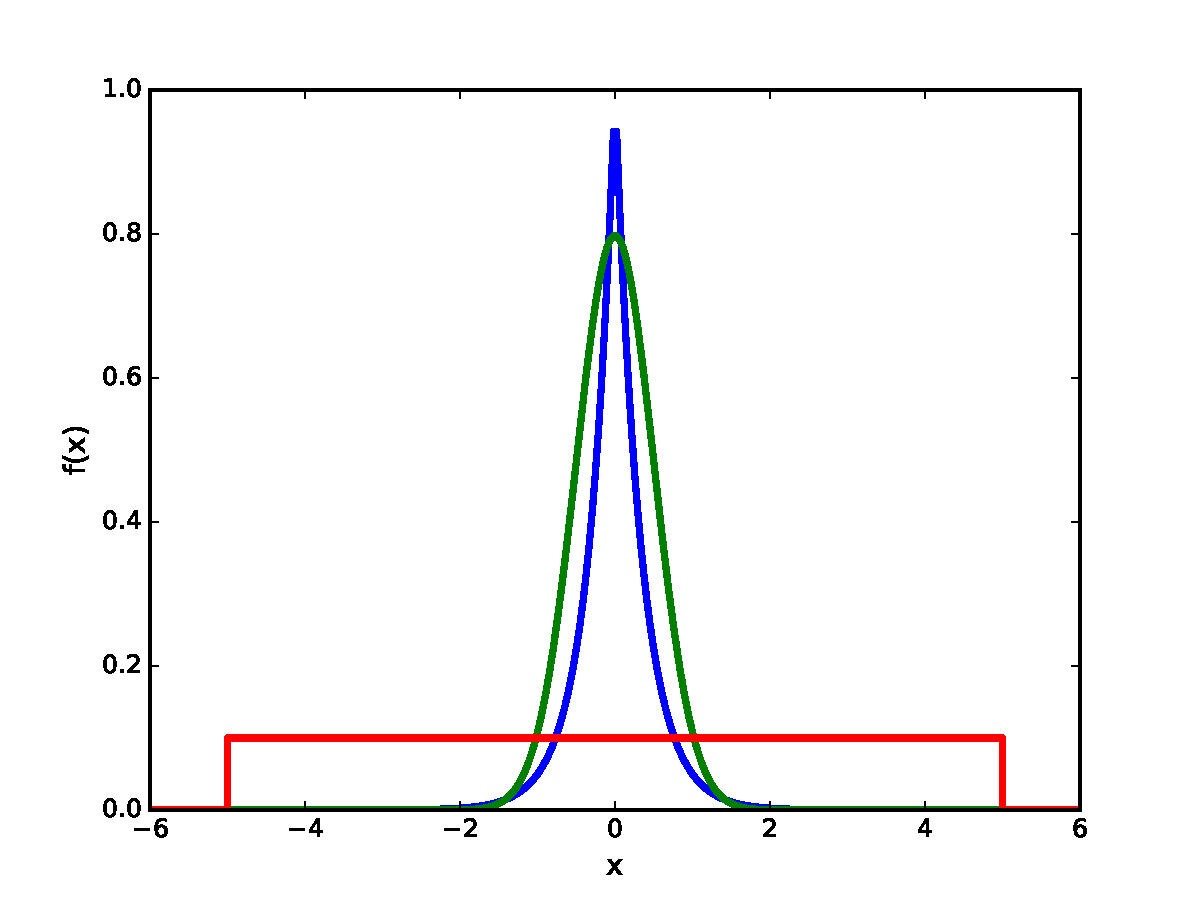
\includegraphics[width=\textwidth]{importanceSampling}
		\caption{A simple importance sampling example (see equation~\ref{eqn:simpleIS}).  The integrand, $f(x)$, is shown in blue, the importance sampling
		distribution is shown in green and, for comparison, the uniform probability density function used in the naive case of no importance sampling is also shown (in red).}
		\label{fig:simpleIS}
  	\end{figure}

  	Table~\ref{tab:simpleIS} clearly shows the value of an importance sampling approach as convergence to the correct result of $1234$ is much faster than when we sampled uniformly.
  	This approach relies on us having some prior knowledge of the behaviour of our integrand in order to select the correct probability density function to use\footnote{More novel approaches whereby the sampling distribution is modified to improve convergence as the Monte-Carlo iterations are calculated, such as the \texttt{VEGAS} algorithm exist but they will not be discussed here.}.
  	A more realistic, and relevant, example of importance sampling comes from the cross-section for the production of a $Z^0$ boson in association with dijets.  The matrix element squared for such a process will have following form upon factoring out the $Z^0$ propagator squared:

  	\begin{equation}
  		|\mathcal{M}_{Z^0+jj}|^2 \sim \left|\frac{1}{p_Z^2 - M_Z^0 + i\Gamma_ZM_Z}\right|^2\times f(\text{QCD, EW})\times g(\text{Kinematic}),
  		\label{eqn:schematicZ}
  	\end{equation}

  	where $p_Z$ is the momentum carried by the $Z^0$ boson, $M_Z$ is its mass, $\Gamma_Z$ is its width and $f(\text{QCD, EW})$ will contain all of the coupling information and $g(\text{Kinematic})$ encodes the remainder of the matrix element.  When using a Monte-Carlo approach to generate events of this kind we can use the schematic of \ref{eqn:schematicZ} to \emph{a priori} select an appropriate probability density function to sample from.  Figure~\ref{fig:breitWigner} shows the squared $Z^0$ propagator.  Obvious comparisons with figure~\ref{fig:simpleIS} can be drawn in the sense that were we to generate events with a uniform spread of values for $p_Z^2$ we would end with a very slow rate of convergence by oversampling areas where the integrand is very small and slowly varying.

	\begin{figure}[htp]
		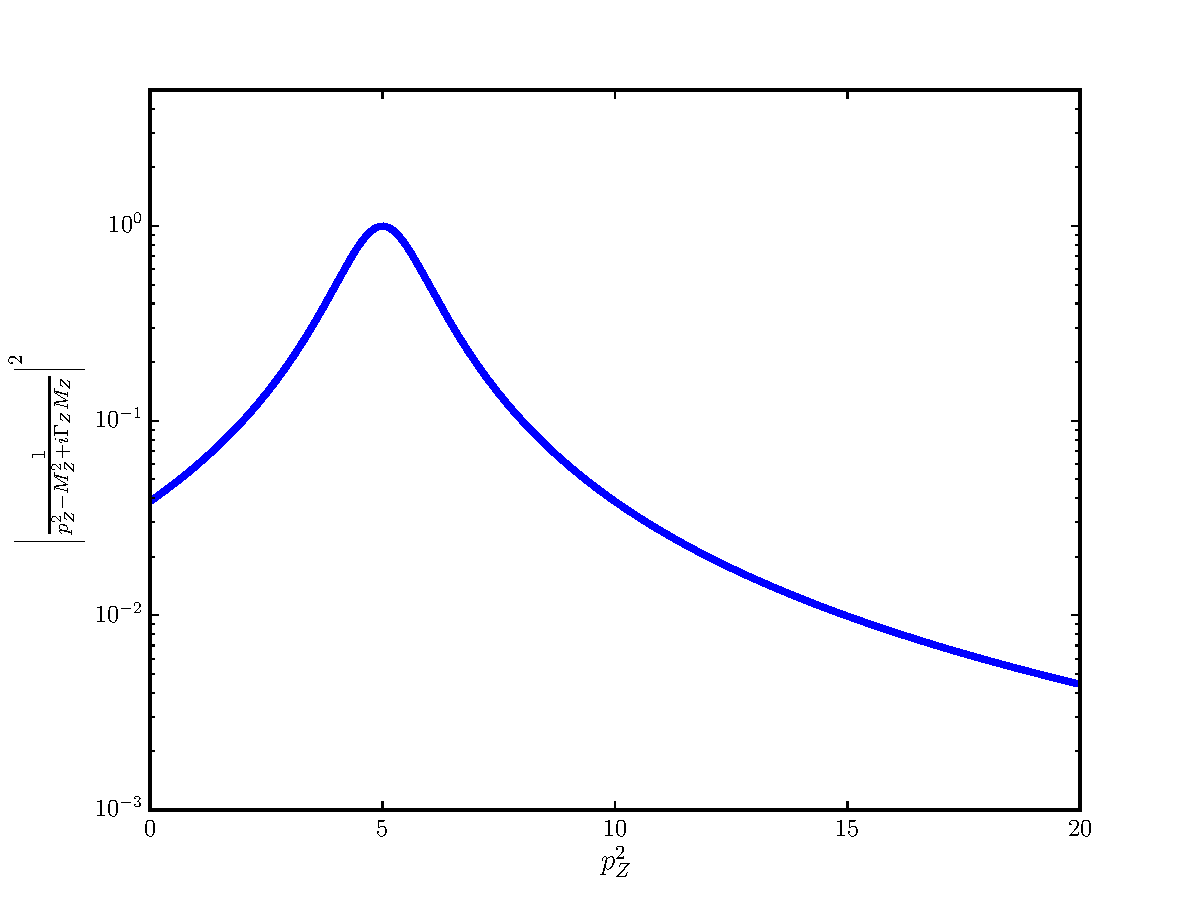
\includegraphics[width=\textwidth]{breitWigner}
		\caption{The absolute value squared of the $Z^0$ propagator for a range of values of the invariant mass squared of the $Z^0$, $p_Z^2$.  We can see it is strongly peaked at the $Z^0$ mass and, as such, is an ideal candidate for using importance sampling.}
		\label{fig:breitWigner}
  	\end{figure}

  	Another good example of importance sampling is found in how we sample the incoming partons in our simulations.  Simple momentum conservation considerations lead us to values for the Bjorken scaling variables of our incoming partons, $x_a$ and $x_b$, and we can use these to intelligently sample the available partons.  The naive way to perform the sum over all possible incoming states would be to uniformly choose a random number corresponding to one of the light quarks, one the light anti-quarks or to a gluon\footnote{By `light (anti-)quarks' we mean all except the top and anti-top.  The parton density functions for these are not available and, even if they were, they would be small enough that we could safely ignore their contribution to cross-sections.}.  We can, however, do better than this by using what we know about how the parton density functions vary with $x_{a/b}$ - figure~\ref{fig:PDFdensities} shows this behaviour as measured by ***who?***.  By choosing to randomly sample then incoming parton types according to the relative values for the parton density functions we can, once again, reduce the variance of our numerical integrations as much as possible.

